% !TEX encoding = UTF-8 Unicode

\documentclass[twocolumn,10pt,a4j]{ltjsarticle}
\usepackage{kougai}

\title{伝統芸能継承問題における小学生向け学習教材の開発}
\author{1932102 永塚 迅一  指導教員 須田 宇宙 准教授}
\date{}
\begin{document}
\maketitle
\section{はじめに}

%背景
日本には今もなお,人々を魅了し感動を与える伝統芸能がある.伝統芸能は,日本舞踊,演劇,演芸,歌,音曲,工芸,芸道の7種類に分けられ,さらにそこから細かく分かれていく.しかし,高齢化や後継者不足により満足に活動することができない問題がある.

茨城県の伝統芸能に「女沼のささら」という獅子舞があり,ささら保存会によって保存継承がなされている.また、地元小学校の運動会では児童がささらを披露する.

%問題点
小学校の運動会で披露するささらは,4年生から6年生の選抜された代表児童を中心に全員参加でささらを踊る.そこでささら保存会が運動会前に,代表児童に数回指導を行うのだが,保存会の人数は年々減ってきており,代表児童に対して十分な指導ができないという問題点がある.

%目的
そこで本研究では,ささらの踊りを学習できる教材を開発し,保存会の教えと併用することでささら代表児童に十分な踊りの知識を提供することを目的とする.

\section{ささら学習教材}
ささら学習教材はQRコードやURLからアクセスして利用できるWeb教材である.本教材で学習することにより,踊りの基礎知識を得ることができる


ささらを踊る際にポイントがあり,小学生の代表児童がよくやってしまう悪い例と正しい例を理解させながら学習していくことが効果的であると考えた.そこで学習教材では,まず保存会の方が実際に踊っている動画を視聴し,その中でポイントごとに番号を表示する.そして,その番号のボタンをクリックすると悪い例,良い例を確認することができる.

構成としては,太鼓のたたき方などの「基本」,実際に運動会で踊る「出羽」「平庭」の3つを選択でき,自分の気になる踊りを学習することができる.例として,「出羽」を選択してポイントの番号1をさらにクリックし,良い例と悪い例の解説ページに遷移する画面を図\ref{fig:ささら}に示す.
\begin{figure}[h]
\begin{center}
 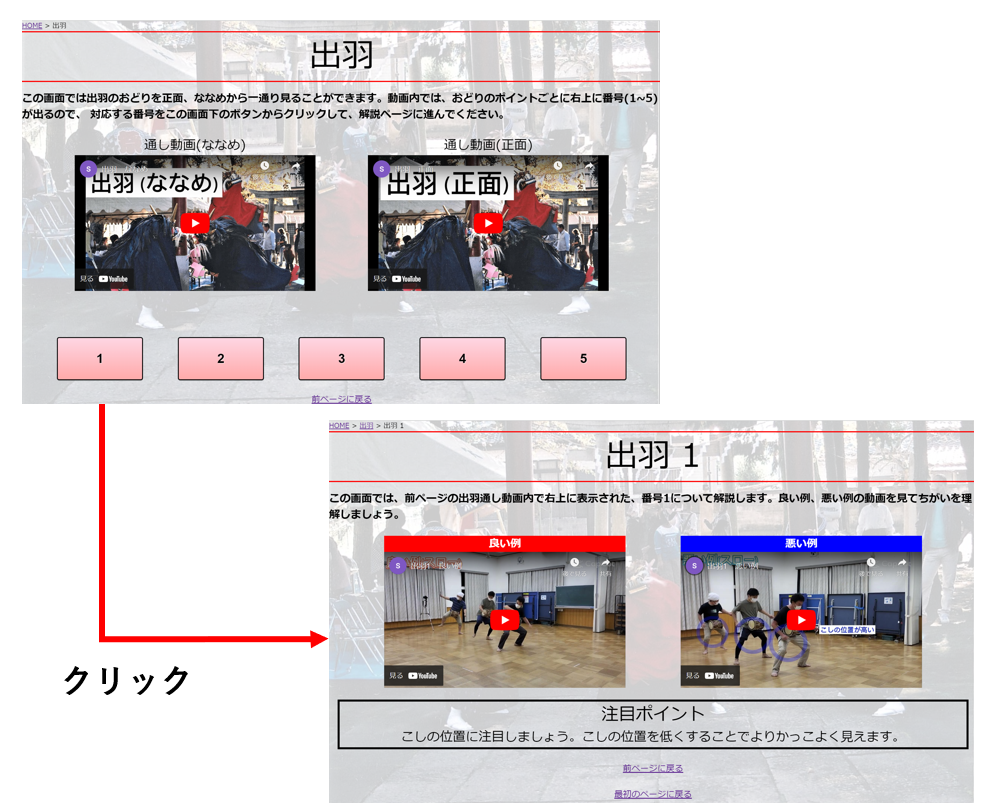
\includegraphics[clip,width=80mm,height=48mm]{figures/kyouzai12.png}
\end{center}
 \caption{ささら学習教材の表示画面例}
 \label{fig:ささら}
\end{figure}

\section{アンケート調査}
本教材の有用性を示すために,小学6年生のささら代表児童5名にアンケート調査を実施した.全9項目に解答してもらい,
「とてもそう思う」「そう思う」「そう思わない」「全くそう思わない」の4択で解答してもらった。
その中で本教材の有用性を示す結果を図\ref{fig:図2},\ref{fig:図3}に示す.「そう思わない」「全くそう思わない」については,解答されなかったので省略した.
\vskip\baselineskip
\begin{figure}[h]
\begin{center}
 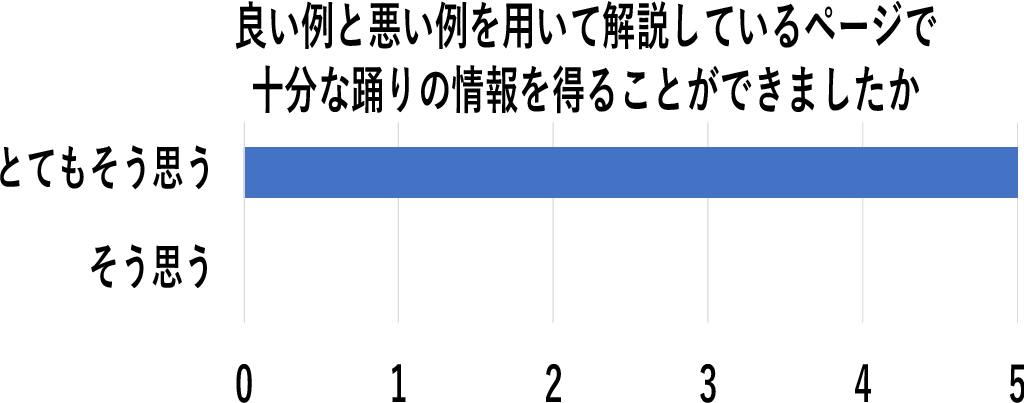
\includegraphics[clip,width=80mm,height=20mm]{figures/zu2.png}
\end{center}
 \caption{アンケート結果1}
 \label{fig:図2}
\end{figure}
\vskip\baselineskip
\begin{figure}[h]
\begin{center}
 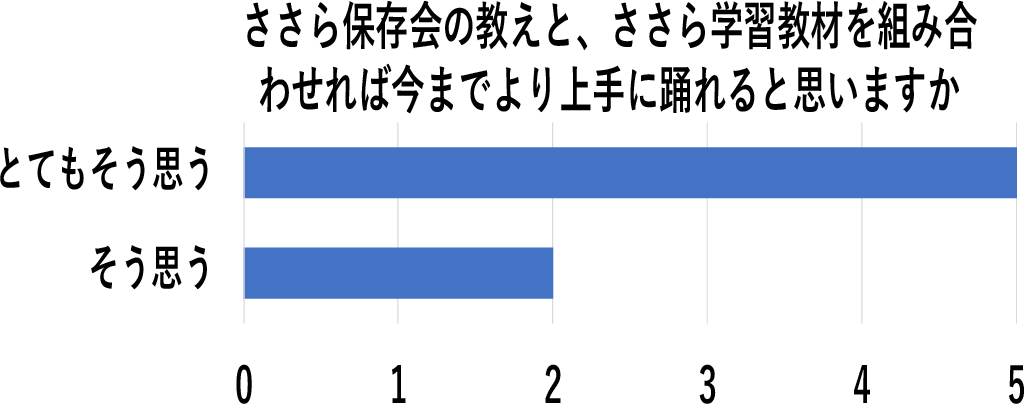
\includegraphics[clip,width=80mm,height=20mm]{figures/zu3.png}
\end{center}
 \caption{アンケート結果2}
 \label{fig:図3}
\end{figure}

図\ref{fig:図2}より,良い例と悪い例を用いて解説すると十分な踊りの知識を得ることが可能なことが分かる.そして図\ref{fig:図3}から本研究の目的を検証したことが分かる.

\section{終わりに}
地元のささらが十分な指導ができていない状況なので,全国の主要な伝統芸能も同じ育成問題をかかえている可能性がある.そこで,良い例,悪い例を用いた学習教材を作成することによって解決の糸口になると考える.

\begin{thebibliography}{99}
\bibitem{suda2018} 古河市 生涯学習課: ``女沼のささら(市指定文化財)/古河市公式ホームページ'', \url{https://bunkashisan.ne.jp/bunkashisan/08_ibaraki/7040.html}, 2022/8/8 参照
\end{thebibliography}

\end{document}